% \AtBeginSection[]{
%     \begin{frame}
%         \frametitle{}
%         \tableofcontents[currentsection]
%     \end{frame}
% }

%%%%%%%%%%%%%%%%%%%%%%%%%%%%%%%%%%%%

\section{Évaluation dans des environnements de jeux coopératifs}

\begin{frame}{Évaluation dans des environnements de jeux coopératifs}

    \begin{block}{Environnements de type Atari}

        \begin{minipage}{0.5\textwidth}
            \centering
            \begin{itemize}
                \item \textquote{Drone swarm - 3rd CAGE Challenge}~\parencite{cage_challenge_3_announcement} (CYB);
                \item \textquote{Pistonball} (PBL)~\parencite{Terry2021};
                \item \textquote{Predator-prey with communication}~\parencite{Lowe2017} (PPY);
                \item \textquote{Knights Archers Zombies}~\parencite{Terry2021}.
            \end{itemize}
        \end{minipage}\hfill
        \begin{minipage}{0.5\textwidth}
            \centering
            \begin{figure}[H]
                \centering
                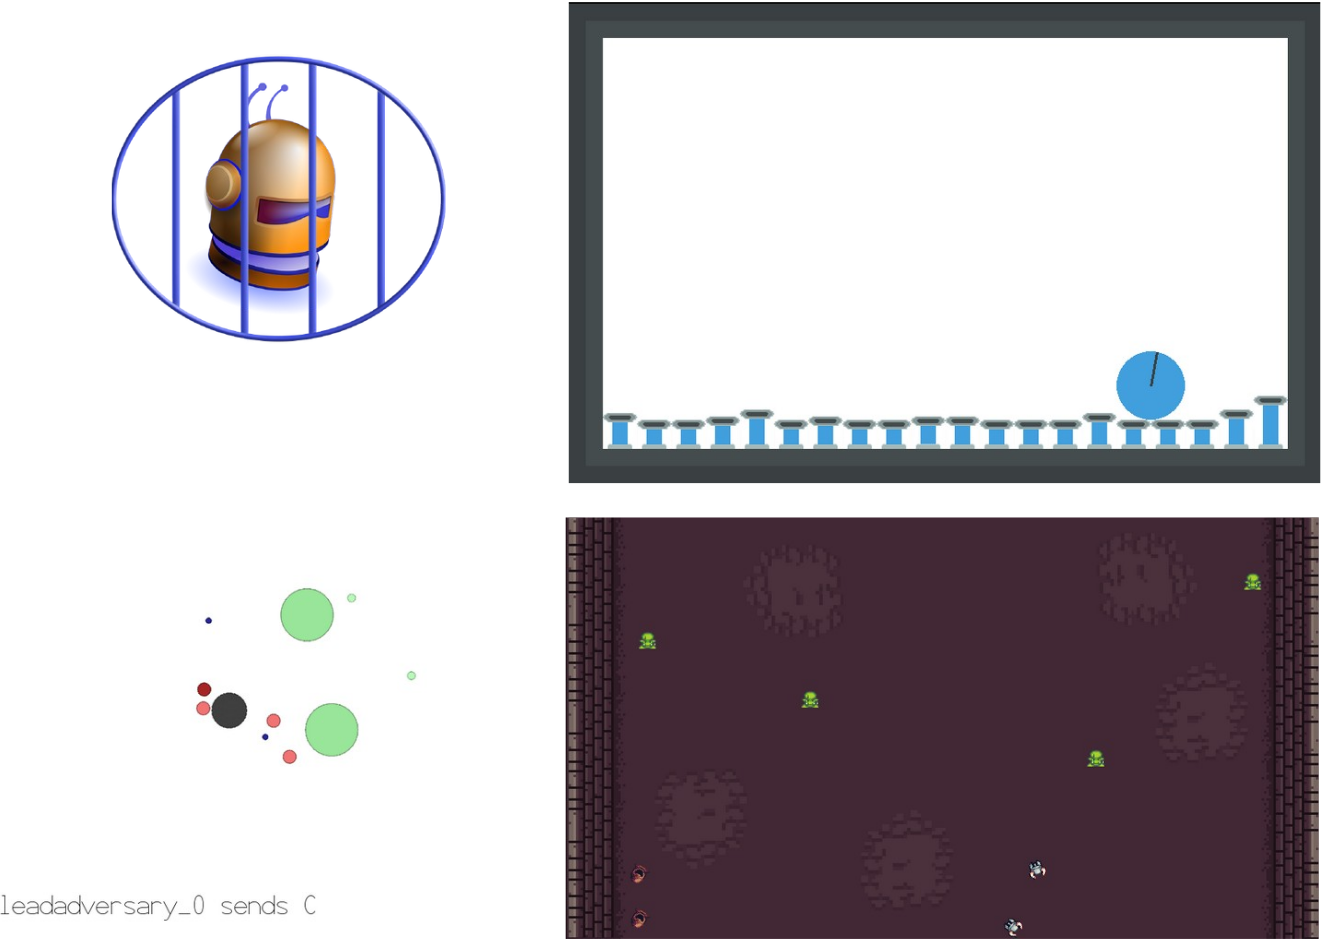
\includegraphics[width=0.5\linewidth]{figures/envs_4x4.png}
                \caption*{Aperçu des environnements sélectionnés : CYB, PBL, PPY et KAZ}
                \label{fig:simulated_environments}
            \end{figure}
        \end{minipage}\hfill

    \end{block}

    \begin{block}{Modes d'application d'AOMEA}
        \begin{itemize}
            \item Sans spécifications organisationnelles (NTS)
            \item Spécifications organisationnelles partiellement contraignantes (PTS)
            \item Spécifications organisationnelles entièrement contraignantes (FTS)
        \end{itemize}
    \end{block}

    $\Longrightarrow$ Évaluation quantitative/qualitative de l'impact sur la performance pendant/après l'entraînement

\end{frame}


\begin{frame}

% Boucle pour afficher toutes les images de frame000.png à frame099.png
\foreach \i in {000, 001, 002, 003, 004, 005, 006, 007, 008, 009, 010, 011, 012, 013, 014, 015, 016, 017, 018, 019, 020, 021, 022, 023, 024, 025, 026} {

    \begin{onlyenv}<\i>
    % \begin{frame}[plain]
        \frametitle{Exemple : Pistonball après entrainement}
        \centering
        \includegraphics[width=0.8\textwidth]{figures/pistonball_frames/frame\i.png}
    % \end{frame}

    \end{onlyenv}

}

\end{frame}

\begin{frame}{Évaluation dans des environnements de jeux coopératifs}{Quelques résultats}

    \begin{columns}

        \begin{column}{0.5\textwidth}
            \begin{figure}[h!]
                \centering
                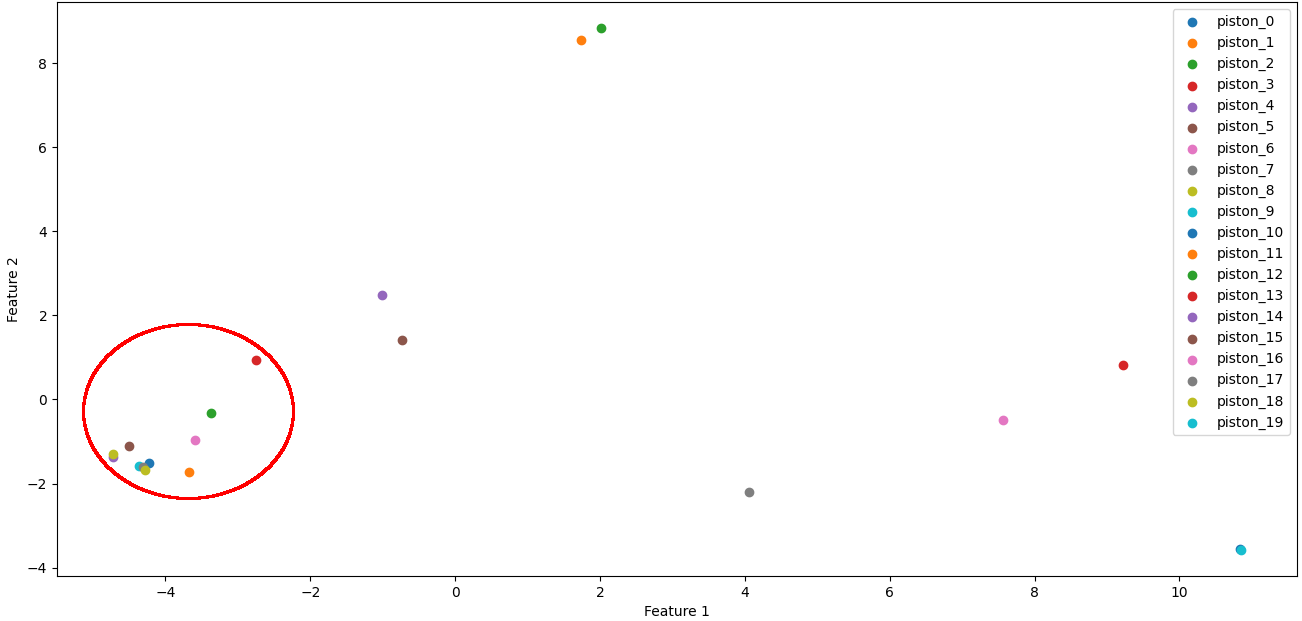
\includegraphics[width=\textwidth]{figures/prahom_pca_analysis.png}
                \caption*{ACP des historiques des agents entraînés dans l'environnement PBL}
                \label{fig:prahom_pca_analysis}
            \end{figure}
        \end{column}

        \hspace{1ex}

        \begin{column}{0.5\textwidth}
            \begin{figure}[h!]
                \centering
                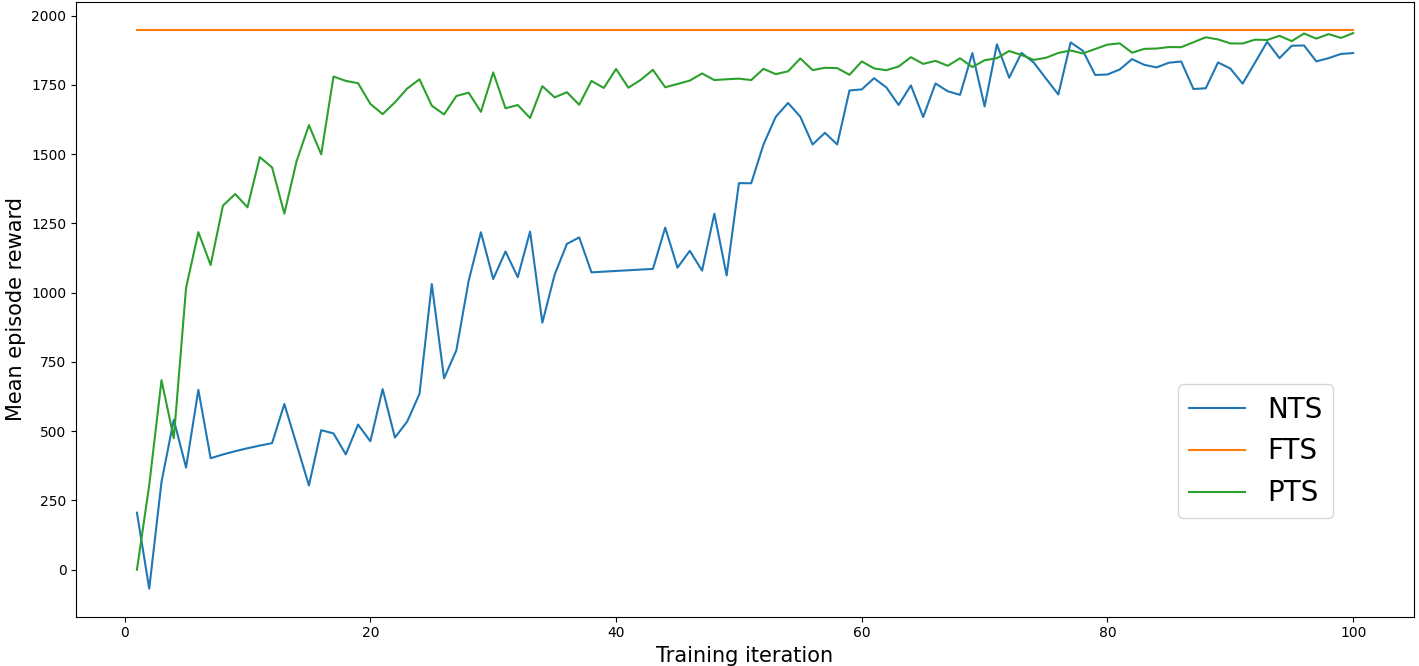
\includegraphics[width=0.95\textwidth]{figures/prahom_learning_curve.png}
                \caption*{Récompense moyenne pour chaque itération dans l'environnement PBL pour les cas NTS, PTS et FTS}
                \label{fig:prahom_learning_curve}
            \end{figure}
        \end{column}

    \end{columns}

\end{frame}

\begin{frame}{Évaluation dans des environnements de jeux coopératifs}{Discussion globale}

    \begin{block}{Impact sur la performance pendant l'entraînement}
        \begin{itemize}
            \item \textbf{Réduction de l'espace de recherche} : le temps de convergence est plus long pour NTS que pour PTS, qui est également plus long que pour FTS;
            \item \textbf{Performance supérieure de NTS} : les politiques des agents entraînés sont conçues spécifiquement pour résoudre le problème;
            \item \textbf{Impact sur la stratégie de résolution} : faible stabilité de performance dans l'environnement CYB $\rightarrow$ absence de stratégies générales par rapport aux autres environnements.
        \end{itemize}
    \end{block}

    \begin{block}{Évaluation qualitative des agents entraînés et spécifications organisationnelles déterminées}
        \begin{itemize}
            \item \textbf{PBL} : partage d'un rôle commun $\rightarrow$ attendu;
            \item \textbf{KAZ} : les archers ont tendance à s'éloigner des zombies, les chevaliers à s'en approcher $\rightarrow$ deux rôles;
            \item \textbf{PPY} : liens d'autorité entre le prédateur leader et les simples prédateurs $\rightarrow$ stratégies collectives pour encercler la proie;
            \item \textbf{CYB} : liens de communication $\rightarrow$ isolement des drones et d'alerte des drones suspectés.
        \end{itemize}
    \end{block}

\end{frame}
